\section{Transitioning to Decentralised Governance}
\label{sect:transition}

The move to automated decentralised governance is irreversible.  In order to mitigate security and other implementation risks, and to ensure that the off-chain and on-chain
processes are sufficiently robust, it is sensible to undertake a number of pilot studies prior to enabling full on-chain automation.

\subsection{On-Chain Pilot}

Initially, pilots can be used where governance decisions are taken off-chain, and then enacted on-chain using the existing manual update process from Shelley/Allegra/Mary/Alonzo.
As part of these pilots, some or all genesis delegate keys could initially be devolved to community members (perhaps in a time-limited way).  This immediately reduces centralisation,
but doesn't enable full autonomy or introduce additional governance checks.

A second pilot could then involve implementing a testnet that can be used to mimic the automated on-chain process.  This has the advantage of allowing the full on-chain automated
process to be tested, with governance decisions enacted on mainnet, without needing to process the hard fork on-chain.  That reduces both timing risk and any risk from failed automation.
The following steps are necessary.

\begin{itemize}
\item
  Stake snapshots must be produced that are to be used in the testnet.  Two snapshots may be needed: one for endorsement and one for voting.  The snapshot must include
  test ada for all those who should be involved in the vote.
\item
  Delegates register on the testnet.
\item
  A formal proposal is prepared and submitted to the testnet.
\item
  Ada holders delegate their vote to registered delegates.
\item
  Delegates vote on whether or not to accept the proposal.
\item
  Assuming the proposal is accepted, it is passed for endorsement (if necessary).
\item
  A proposal that is accepted and endorsed is enacted on the testnet.
\item
  Assuming it has been enacted on the testnet and there are no security or other concerns, an identical proposal is submitted on mainnet and the usual manual steps are
  followed to enact the proposal.
\end{itemize}

It is recommended that the pilot proposal be for either some specific funds transfer, or for some simple parameter update, rather than for a protocol version.

\subsection{Off-Chain Governance}

The full governance chain will also need to be tested on an end-to-end basis.  An idea will need to be discussed and a proposal submitted for formal off-chain voting.  Assuming it is not rejected,
the proposal will need to be implemented, checked for any security issues, passed to an implementor group, checked and recorded by the CIP editors, then submitted on-chain.
Depending on timings, this can be done either through the initial on-chain pilot, though the manual process, or through the on-chain automated enactment process.

\begin{figure}
  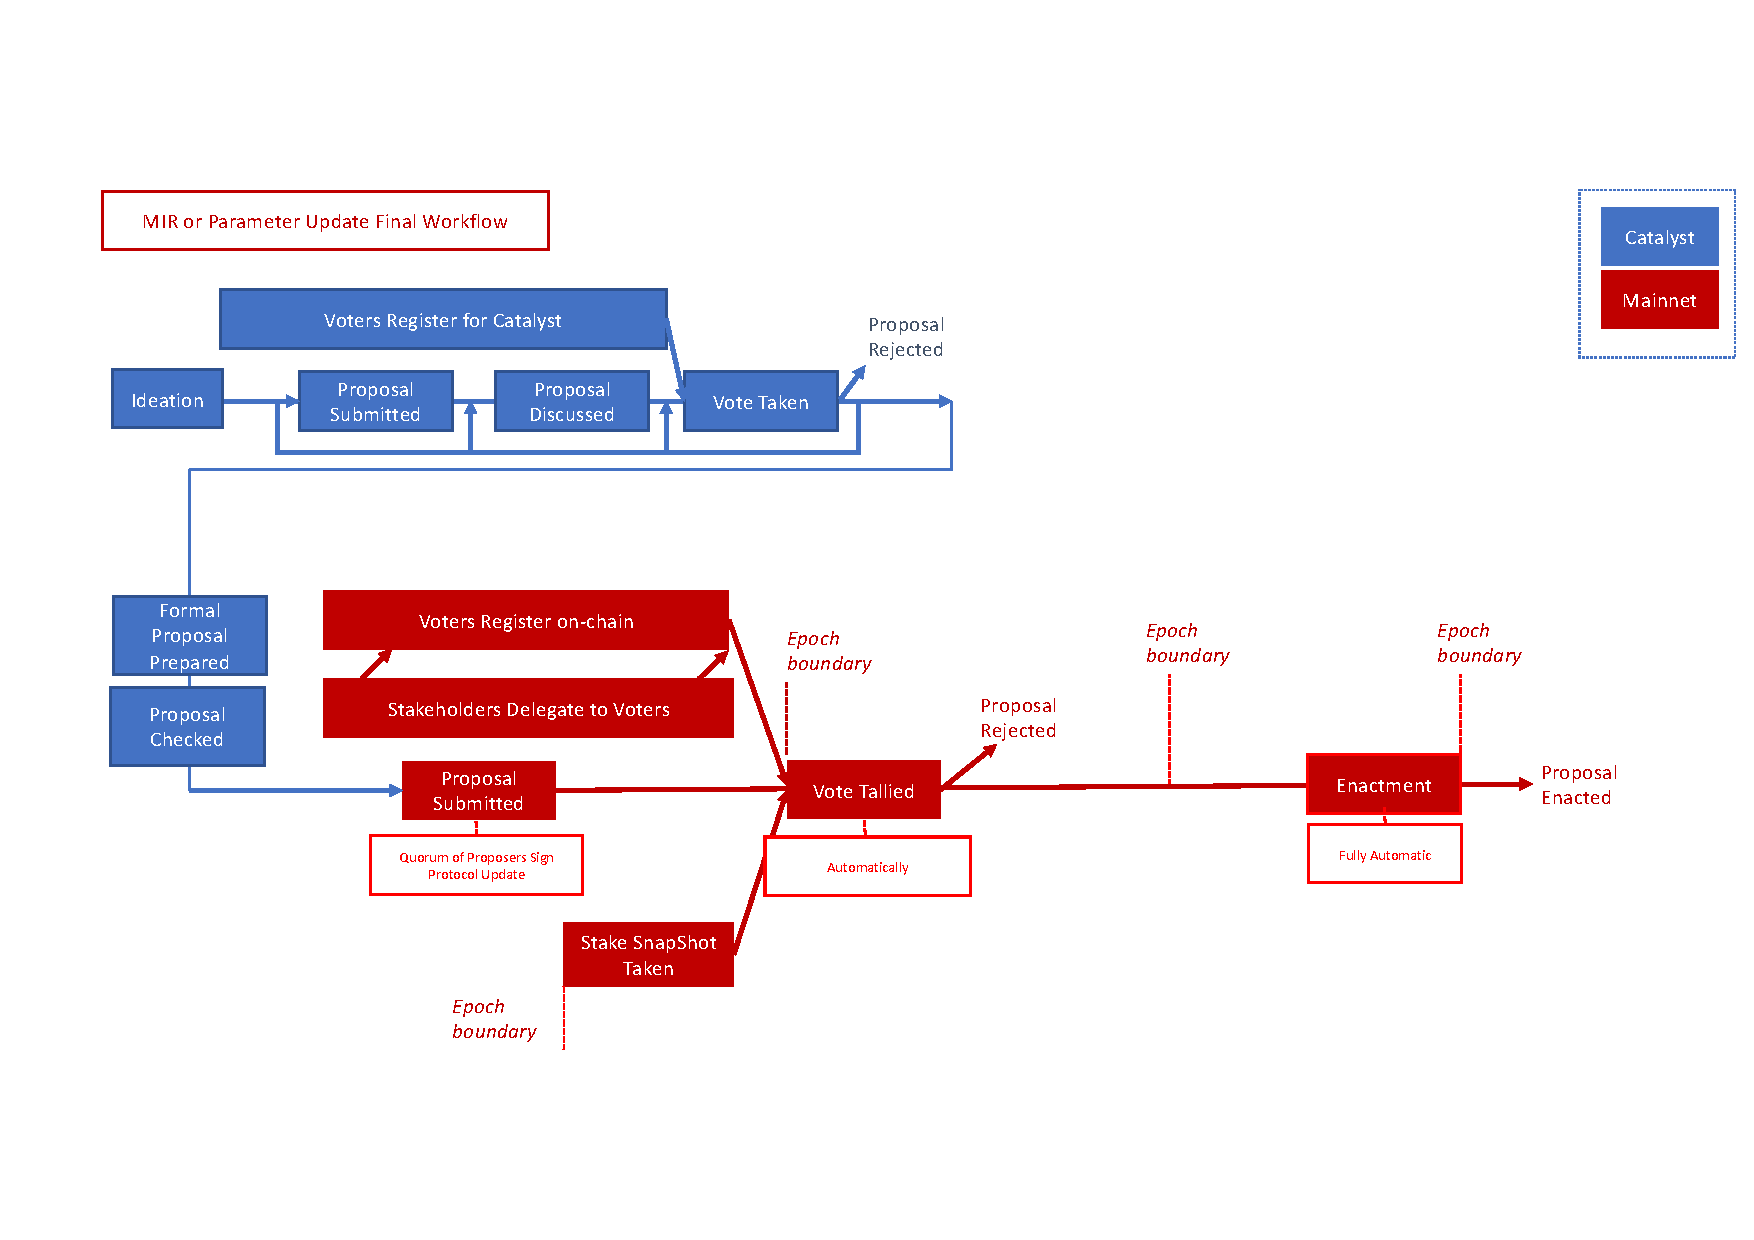
\includegraphics[trim=0 90 0 80,clip,width=\textwidth]{Workflow3}
  \caption{Example Workflow: Funds Transfer (MIR) or Simple Parameter Value Update, showing off-chain delegation and voting simulation steps for initial pilot}
  \label{fig:workflow-mir2}
\end{figure}

\begin{figure}
  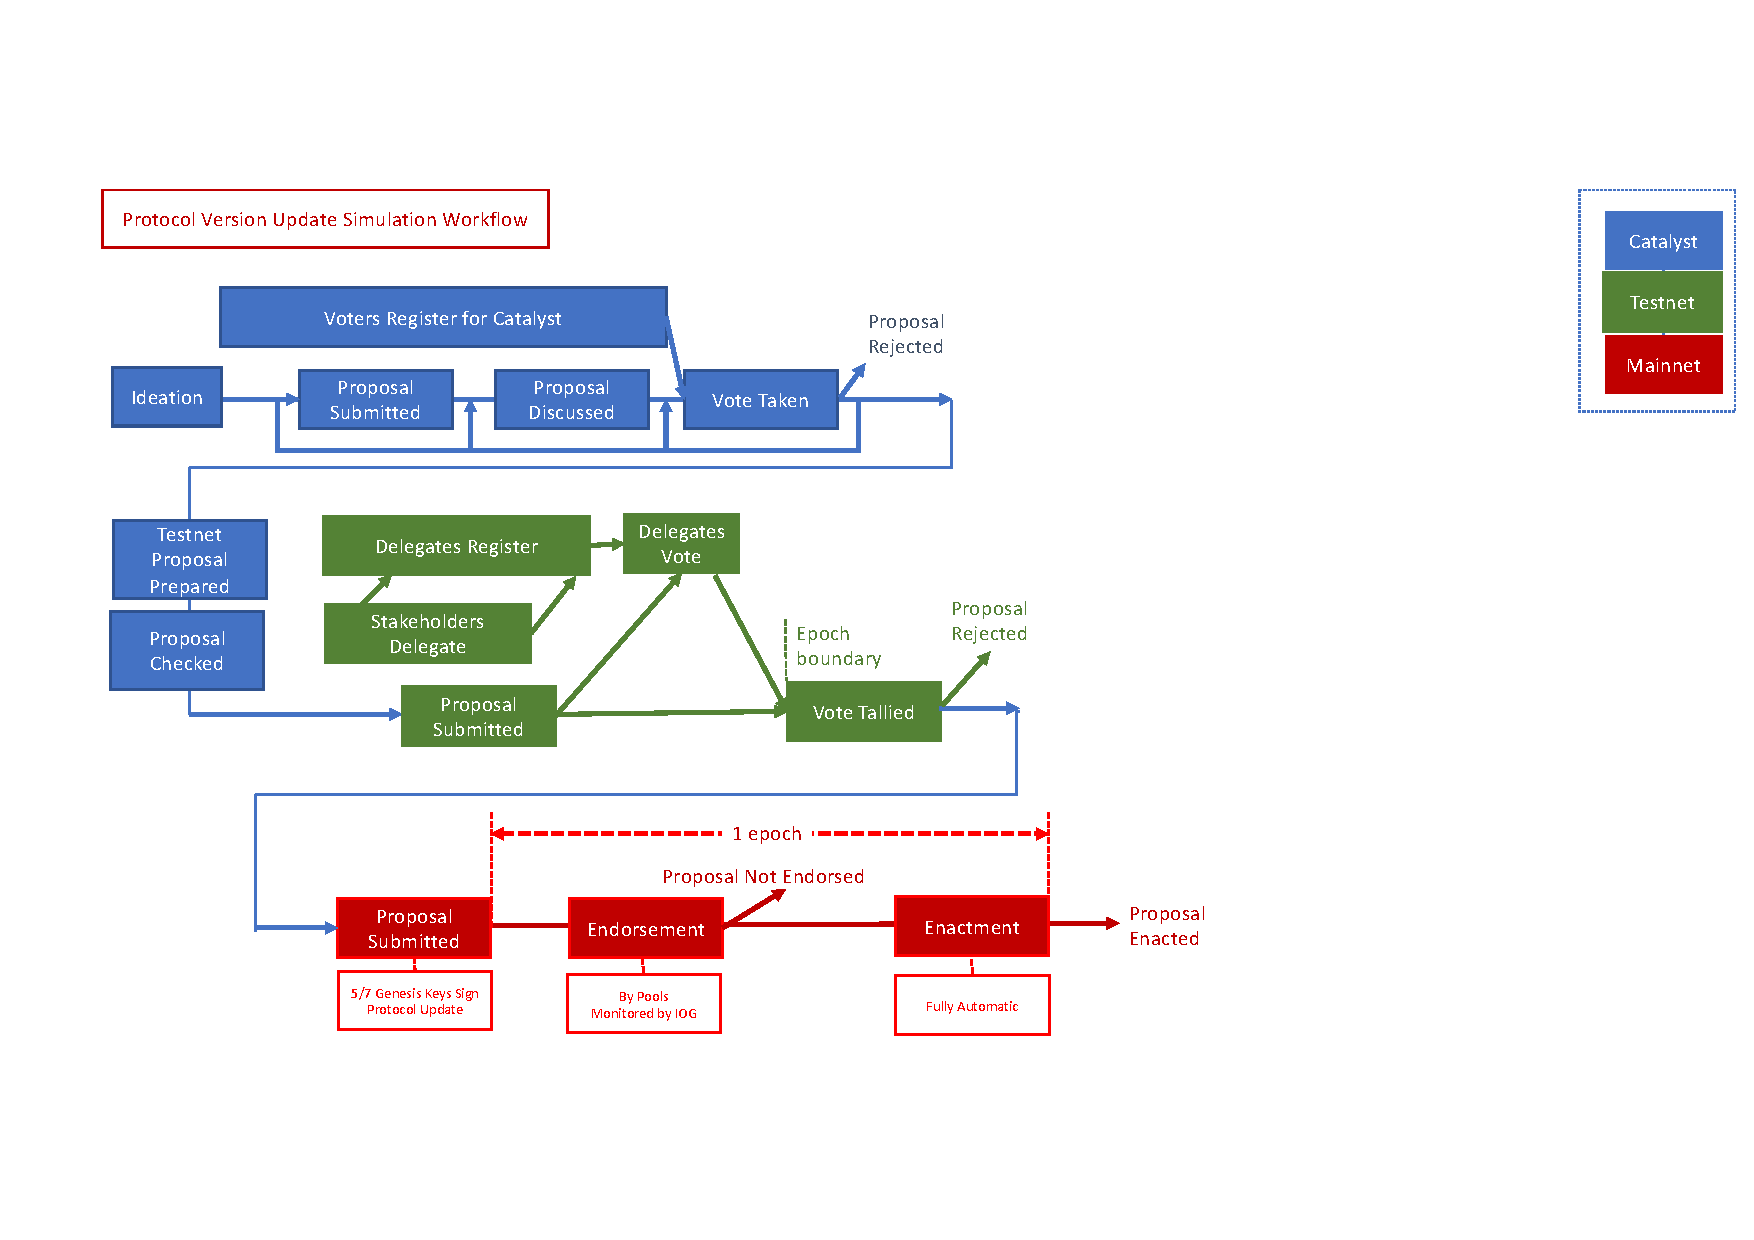
\includegraphics[trim=0 90 0 80,clip,width=\textwidth]{Workflow4}
  \caption{Example Workflow: Protocol Version Update (Hard Fork), showing off-chain delegation and voting simulation steps for initial pilot}
  \label{fig:workflow-hf2}
\end{figure}

\subsection{Workflows for Accelerating Early Governance Pilots.}
\label{sect:pilot-workflows}

Figures~\ref{fig:workflow-mir2}-\ref{fig:workflow-hf2} show the corresponding  workflows that could be used if desired,
for initial pilots.  The off-chain process is identical in all cases, but the on-chain delegation process is mimicked precisely on a testnet, rather than performed
on-chain.  Accepted proposals are then passed for manual submission and enactment on-chain.  This will allows early testing and tuning of governance mechanisms without
irrevocably changing the on-chain governance process, so permitting more rapid deployment of decentralised governance with reduced implementation and automation risk.

\subsection{Genesis Keys/Genesis Delegates}

Once the protocol has been updated to include the on-chain PUP mechanisms, the
genesis keys and their delegates will cease to have any governance power.  The
chain can only legitimately be continued through the decentralised governance
mechanism.  Once the chain has been extended, and it is decided that the chain
will never need to be reverted, the keys may safely be destroyed.
